\chapter{Preliminarii}

\section{Noțiuni fundamentale privind învățarea prin întărire}
\subsection{Definirea problemei de învățare prin întărire}

Învățarea prin întărire reprezintă paradigma de învățare automată din cadrul domeniului inteligenței artificiale, în care un agent învață să ia decizii optime prin interacțiunea cu un mediu, primind recompense sau penalizări pentru acțiunile sale, cu scopul obținerii unei politici de acționare optime ce maximizează recompensa obținută \cite{reinforcement_learning_book}.

Imaginați-vă un copil care învață să meargă pe bicicletă. Nu există un manual cu instrucțiuni precise sau un set de date cu "mișcări corecte" etichetate. În schimb, copilul face încercări repetate, primește feedback imediat (cade sau reușește să mențină echilibrul), și gradual își ajustează comportamentul pentru a obține rezultate tot mai bune. Acest proces natural de învățare prin experiență directă este exact ceea ce încearcă să modeleze învățarea prin întărire.

Avantajele paradigmei învățării prin întărire sunt multiple și se pot deduce imediat. O scurtă observare și generalizare a problemelor din lumea reală ne va arăta că următoarele motive îngreunează abilitatea de a genera un algoritm potrivit, fapt pentru care este de preferat utilizarea unui sistem adaptabil și dinamic:
\begin{enumerate}
    \item \textbf{Lipsa etichetelor explicite}: În multe contexte și medii politica optimă este greu de definit sau nu poate fi concretizată într-o formă aplicabilă, fapt pentru care putem doar deduce dacă rezultatul final a fost unul dezirabil sau nu, astfel nemaiavând nevoie de o etichetare manuală înainte de antrenare.
    \item \textbf{Natura secvențială a deciziilor}: Deciziile nu sunt independente - o acțiune luată acum va influența situațiile viitoare și opțiunile disponibile
    \item \textbf{Feedback întârziat}: Consecințele unei acțiuni se pot manifesta într-un plan îndepărtat, făcând dificilă atât previziunea cu efectele imediate cât și încercarea de disipare a consecințelor viitoare.
    \item \textbf{Medii dinamice}: Efectuarea unei acțiuni poate avea consecințe nefaste în cadrul similitudini dintre două stări consecutive, determinând un avantaj clar posibilitatea de generalizare și ajustare constantă.
\end{enumerate}

Formal, problema poate fi modelată ca un proces de decizie Markov (Markov Decision Process, MDP), definit prin tuplul $(S, A, P, R, \gamma)$ \cite{markov_decision_process}, unde:
\begin{itemize}
    \item $S$ = spațiul stărilor din mediu (un set finit sau infinit al tuturor stărilor accesibile din mediu)
    \item $A$ = spațiul acțiunilor (un set de acțiuni prin care agentul poate interacționa cu mediul)
    \item $P: S\times A \times S \xrightarrow{} [0, 1] $ = funcția de tranziție (probabilitate efectuării acțiunii $a \in A$ în starea $s \in S$, ajungând în starea $s\prime \in S$)
    \item $R: S \times A \xrightarrow{} \mathbb{R}$ = funcția de recompensă (obținute în urma efectuării acțiunii $a \in A$ în starea $s \in S$)
    \item $\gamma \in [0, 1]$ = factorul de discount pentru recompense viitoare (cât de mult vrem să ținem cont de rezultatele viitoare comparativ cu cele imediate).
\end{itemize}

Pentru simplitatea scrierii vom considera că atunci când notăm o acțiune $a \in A$, o stare $s \in S$, o probabilitate $p \in S\times A \times S \xrightarrow{} [0, 1]$ sau o recompensă $r \in S \times A \xrightarrow{} \mathbb{R}$ vom scrie doar literele mici, fără a mai preciza domeniul funcției.

Proprietatea unui proces Markov stipulează că probabilitatea de tranziție către o stare viitoare nu depinde de toate stările anterioare, ci doar de starea și acțiunea curentă:
\begin{center}
$P(s_{t+1} | s_t, a_t, s_{t-1}, a_{t-1}, ..., s_0, a_0) = P(s_{t+1} | s_t, a_t)$.
\end{center}

Această proprietate ne va fi de foarte mare folos prin gradul de simplitate al implementării, reducând dramatic complexitatea algoritmilor. Generalizarea și convergența matematică sunt de asemenea îmbunătățite, permițând și chiar asigurând existența unui optim global în cadrul unui mediu binedefinit.

\begin{figure}[H]
\centering
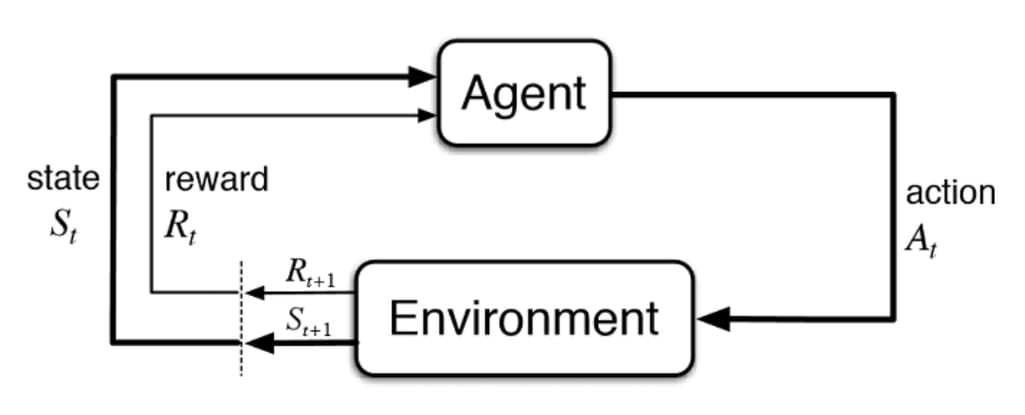
\includegraphics[width=10cm]{images/reinforcement_learning_scheme.jpg}
\caption{Reprezentarea vizuală a unui PDM \cite{reinforcement_learning_scheme_image}}
\end{figure}

\subsection{Funcții de valoare și politici optime}
\subsubsection{Funcția de politică a agentului}
În contextul mediului definit, \textbf{politica} (policy) reprezintă "strategia" pe care o urmează agentul în cazul determinării acțiunii potrivite. Aceasta concretizează mecanismul probabilistic parcurs de agent în cadrul unei "rute" de stări.

Aceasta poate fi de două feluri:
\begin{enumerate}
    \item \textbf{Politica deterministă}: $\pi:S \xrightarrow{} A$
    \begin{itemize}
        \item Mapează fiecare acțiune la o singură stare
        \item Exemplu: Când pică bicicleta, o ridic.
    \end{itemize}
    \item \textbf{Politica stocastică}:  $\pi:S \times A \xrightarrow{} [0, 1]$
    \begin{itemize}
        \item Definește o distribuție de probabilitate peste acțiuni pentru fiecare stare
        \item $\pi(a|s)$ = probabilitatea de a alege acțiunea $a$ în starea $s$
        \item Exemplu: Atunci când se murdărește bicicleta, 90\% din timp o voi spăla imediat, iar 10\% din timp o voi curăța a doua zi.
    \end{itemize}
\end{enumerate}

Politicile stocastice permit agentului să exploreze diferite acțiuni ceea ce cresc șansele de descoperire a unei politici optime, care să poată fi exploatată ulterior. Totodată, ele conferă și robustețe făcând predicția comportamentului mai puțin anticipabilă de către adversari.

\subsection{Evaluarea politicilor: Funcțiile de valoare}
Pentru a determina cât de bună este o anumită politică, avem nevoie de o modalitate de măsură a performanței acesteia. Cu ajutorul funcțiilor de valoare, putem defini o metrică ce estimează gradul de utilitate al unei situații sau acțiuni raportat la ajutorul oferit atingerii scopului predefinit.

Va trebui mai întâi să definim noțiunea de \textbf{episod}, care reprezintă secvența ordonată temporal al tuplurilor de acțiune și stare, pe care agentul o întreprinde pornind de la o stare inițială până la o stare terminală, $t$.
\begin{center}
    $s_0a_0, s_1a_1, \space ..., s_ta_t$
\end{center}

Funcția de valoare a stării (State Value Function) $V^\pi(s)$ reprezintă recompensa totală așteptată pe care o poate obține agentul pornind din starea $s$ și urmând politica $\pi$ pentru tot restul episodului.
\begin{center}
    $V^\pi(s) = E_\pi[\sum_{t=0}^\infty \gamma^t R_{t+1} | S_0 = s]$, unde:
\end{center}
\begin{itemize}
    \item \textbf{$E_\pi$} este valoarea așteptată, urmărind politica $\pi$
    \item \textbf{$\gamma ^ t$} este factorul de discount aplicat recompensei de la timpul $t$
    \item \textbf{$R_{t+1}$} este recompensa primită la timpul t+1
    \item \textbf{$S_0 = s$} este condiționarea că începem din starea $s$.
\end{itemize}

Scrierea extinsă a lui $V^\pi(s)$ ne arată de fapt că acesta doar urmărește care este rezultatul final al deciziilor noastre. Factorul $\gamma$ ne ajută să valorificăm mai mult recompensele imediate, în detrimentul celor viitoare, în practică acesta are o valoare cuprinsă între 0.99 și 0.95, depinzând de context.
\begin{center}
    $E_\pi[R + R\gamma + R\gamma^2 + \space ...]$
\end{center}

Funcția de valoare acțiune-stare (Action-Value Function/Q-Function) reprezintă recompensa totală așteptată prin luarea acțiunii $a$ în starea $s$, urmată de aplicarea politicii $\pi$ pentru restul episodului.
\begin{center}
    $Q^\pi(s,a) = E_\pi[\sum_{t=0}^\infty γ^t R_{t+1} | S_0 = s, A_0 = a]$, unde:
\end{center}
\begin{itemize}
    \item la fel ca mai sus, regăsim aceiași termeni, doar că vom condiționă acum utilizarea acțiunii $a$ în starea $s$ prin $S_0 = s, A_0 = a$.
\end{itemize}

Diferența dintre cele două este că funcția $Q$ ne permite să alegem ce acțiune să fie utilizată prima dată, după care ambele funcții urmăresc evoluția evenimentelor alese prin politica $\pi$. În practică preferăm să utilizăm funcția $Q$ deoarece ne permite să alegem cea mai bună acțiune într-o stare, astfel ajungând la un rezultat optim. Relația dintre cele două este că funcția de valoare $V$ este media ponderată după probabilitate de a acționa în starea $s$ cu acțiunea $a$, conform cu funcția $Q$:
\begin{center}
    $V^\pi(s) = \sum_a \pi(a|s) Q^\pi(s,a)$
\end{center}

\subsection{Ecuația Bellman: Principiul optimizării dinamice}
Ecuația Bellman este cea mai importantă relație matematică oferind o modalitate de a exprima valorile în termeni recursivi. Ecuația spune că valoarea unei stări (sau a unei combinații de stare-acțiune) este egală cu recompensa imediată așteptată plus valoarea ponderată de discount al situației următoare.

\begin{equation}
V^\pi(s) = \sum_a \pi(a|s) \sum_{s'} P(s'|s,a)[R(s,a,s') + \gamma V^\pi(s')]
\label{eq:bellman_v}
\end{equation}

\begin{equation}
Q^\pi(s,a) = \sum_{s'} P(s'|s,a)[R(s,a,s') + \gamma \sum_{a'} \pi(a'|s') Q^\pi(s',a')]
\label{eq:bellman_q}
\end{equation}

\subsection{Politici optime}
Politica optimă $\pi^*$ este cea care maximizează valoarea așteptată pentru toate stările posibile.

\begin{equation}
    \pi^* = \arg\max_\pi V^\pi(s) \text{ pentru toate } s \in S
\label{eq:optim_pi}
\end{equation}

Pentru orice proces de decizie Markov finit, există cel puțin o politică optimă deterministă $\pi^*$. Deși pot exista mai multe politici optime, funcția de valoare optimă $V^*(s)$ este unică pentru fiecare stare $s$, toate politicile optime având aceeași funcție de valoare $V^*(s) = V^{\pi^*}(s)$.

Utilizând rezultatele de mai sus \ref{eq:bellman_q}, \ref{eq:bellman_v}, \ref{eq:optim_pi}, putem construi ecuațiile Bellman pentru politica optimă:
\begin{equation}
    V^*(s) = \max_a \sum_{s\prime} P(s\prime|s,a)[R(s,a,s\prime) + \gamma V^*(s\prime)]
\label{eq:bellman_v_optim}
\end{equation}

\begin{equation}
    Q^*(s,a) = \sum_{s\prime} P(s\prime|s,a)[R(s,a,s\prime) + \gamma \max_{a\prime} Q^*(s\prime,a\prime)]
\label{bellman_q_optim}
\end{equation}

Astfel, conform \ref{bellman_q_optim} și \ref{eq:bellman_v_optim} putem extrage politica optimă cu ajutorul funcției $Q$ optime, un rezultat foarte important pentru progresul curentei lucrări. Odată determinată funcția $Q$ optimă $Q^*(s, a)$, obținerea politicii optime devine trivială, alegând mereu cea mai mare valoare a funcției $Q$ în fiecare stare.

\begin{equation*}
    \pi^*(s) = \arg\max_a Q^*(s,a)
\end{equation*}